% !Mode:: "TeX:UTF-8"
\documentclass[QAofGroup.tex]{subfiles}
\begin{filecontents*}{mdframed-example.tex}
\documentclass{article}
\usepackage[UTF8]{ctex}
\usepackage[framemethod=tikz]{mdframed}
\usepackage{listings}
\usetikzlibrary{calc,arrows,shadings,shadows}
\begin{document}
	\definecolor{DarkBlue}{rgb}{.11,.23,.60}
	\mdfdefinestyle{commandline}%
	{leftmargin=5pt, rightmargin=10pt, innerleftmargin=15pt,
		middlelinecolor=DarkBlue,
		middlelinewidth=2pt,
		frametitlerule=false,
		backgroundcolor=black!10!white,
		frametitle={Command Window},
		frametitlefont={\normalfont\sffamily\color{white}\hspace{-1em}},
		frametitlebackgroundcolor=DarkBlue,
		singleextra={\draw[black!20,line width=12pt]
			($(O)+(7pt,1pt)$) -- ($(O|-P)+(7pt,-\mdfframetitleboxtotalheight)-(0,1pt)$);
			\node[inner sep=0pt, color=black]at ($(O)+(7pt,9pt)$)%
			{$\scriptstyle f\!x$}; },
		nobreak,
	}
	\lstnewenvironment{script}{%
		\lstset{language=Matlab, basicstyle=\tiny\ttfamily, breaklines=true,%
			aboveskip=0pt,belowskip=0pt}}{}
	\surroundwithmdframed[style=commandline]{script}
	
	\begin{script}
		>> help sin
		sin Sine of argument in radians.
		sin(X) is the sine of the elements of X.
		
		See also asin, sind.
		
		Overloaded methods:
		sdpvar/sin
		codistributed/sin
		gpuArray/sin
		
		Reference page in Help browser
		doc sin
		>>
	\end{script}
\end{document}	
\end{filecontents*}
\begin{filecontents*}{AutoFrownSim.tex}
\documentclass{article}
\usepackage[UTF8]{ctex}
\usepackage{ifthen} 
\usepackage{amsmath,bm}
\usepackage{tikz}
\usepackage{scalerel}
\usepackage{stackengine}
\stackMath
%\stackText
\newcommand\reallywidefrown[1]{%
	\stackon[0.5pt]{#1}{%
		\stretchto{%
			\scaleto{%
				\scalerel*[\widthof{#1}]{\mkern-1.5mu\frown\mkern-2mu}%
				{\rule[-\textheight/2]{1ex}{\textheight}}%
			}{\textheight}%
		}{0.8ex}}%
}
\newlength{\lmax}%
\newlength{\lfenzi}%
\newlength{\lfenmu}%
\newcommand\reallywidesim[2]{%
	\savestack{\fenzi}{\(#1\)}%
	\savestack{\fenmu}{\(#2\)}%
	\settowidth{\lfenzi}{\fenzi}%
	\settowidth{\lfenmu}{\fenmu}%
	\ifthenelse{\lengthtest{\lfenzi > \lfenmu}}
	{\setlength{\lmax}{\lfenzi}}
	{\setlength{\lmax}{\lfenmu}}
	\stackon[0.5pt]{\fenmu}{\stackunder[0.5pt]{\fenzi}{%
			\stretchto{%
				\scaleto{%
					\scalerel*[\lmax]{\mkern-1.5mu\sim\mkern-2mu}%
					{\rule[-\textheight/2]{1ex}{\textheight}}%
				}{\textheight}%
			}{1ex}}}%
}
\parskip 1ex
\begin{document}
\[
  \reallywidefrown{zbcdefghi},\qquad 
  \reallywidefrown{zbcdefg},\qquad  
  \reallywidefrown{zbcde},\qquad  
  \reallywidefrown{zbc},\qquad  
  \reallywidefrown{zb},\qquad 
  \reallywidefrown{\Shortstack{\sin z}} = 0
\]
\[
  \reallywidesim{r_1}{r_2},\qquad 
  \reallywidesim{r_1\leftrightarrow r_2}{r_3\div 2 },\qquad 
  \reallywidesim{r_1\leftrightarrow r_2}{r_3\div 2, r_1\leftrightarrow r_2},\qquad 
  \reallywidesim{r_1\leftrightarrow r_2, r_1\leftrightarrow r_2}{r_3\div 2}
\]

也可以使用Tikz来绘制贝赛尔曲线, 但是不便于自适应宽度.
\[
  \begin{array}{@{}c@{}}
    \bm{r_1\leftrightarrow r_2}\\
    
\begin{tikzpicture}
      \draw[line width=1pt] (0,0) .. controls(.5,.11)..(1,0)
          ..controls(1.5,-.15) .. (2,0);
    \end{tikzpicture}\\[-.5ex]
    \bm{r_3\div 2}
  \end{array}
\]
\end{document}
\end{filecontents*}
\begin{document}
%-=-=-=-=-=-=-=-=-=-=-=-=-=-=-=-=-=-=-=-=-=-=-=-=
%
%	CHAPTER
%
%-=-=-=-=-=-=-=-=-=-=-=-=-=-=-=-=-=-=-=-=-=-=-=-=

%%================================================================
\chapter{20180502}\label{ch180502}
%----------------------------------------------------------------------------------------
\begin{qst}\label{Q2018050201}
环境:Windows, TeXLive2017, TeXstudio, pdflatex, UTF8

报错:未定义控制序列\mtl{\end{script}}

代码来源:mdframed帮助文档第16页.\index{mdframed}
\end{qst}
\ans 那个例子调用mdframed宏包时需要指定\mtl{framemethod=tikz},
tikz需要计算之类的, 还需要调用相应的库
\mt{\usetikzlibrary{calc,arrows,shadings,shadows}}

可以参照这样的例子:
\inputminted[fontsize=\normalsize,linenos,breaklines]{tex}{mdframed-example.tex}
\ifcompile\immediate\write18{xelatex mdframed-example.tex}\fi
\begin{center}
	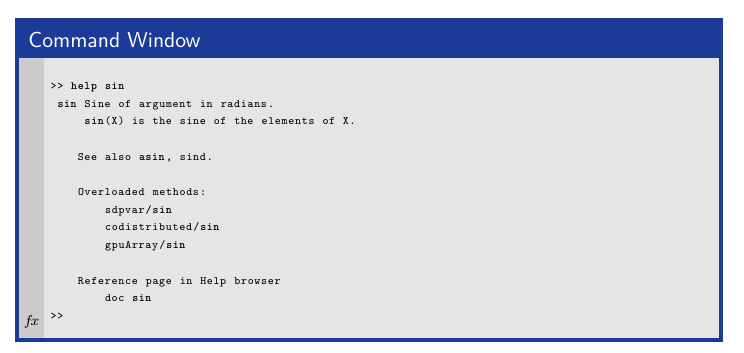
\includegraphics[width = 1\linewidth]{pic18}%{mdframed-example.pdf}
\end{center}

\begin{qst}\label{Q2018050202}
 使用comment环境总是出错, 好像需要把 \mtl{\begin{comment}} 和 \mtl{\end{comment}} 之后都预留空格才行.\index{comment}
\end{qst}
\ans 问题不在这里, 那个comment的问题出在宏包顺序上, tcolorbox和verbatim需要在comment之后, 只要将comment宏包调用放到前面就好了.

\begin{qst}\label{Q2018050203}
 公式编号默认在右侧, 让这些编号移动到左侧,加什么命令啊?\index{fleqn}
\end{qst}
\ans \mtl{\documentclass} 加 fleqn 选项.

\begin{qst}\label{Q2018050204}
	上下积分符号怎么写?\index{上下积分}
\end{qst}
\ans 这种只有少数几个覆盖字符集大的数学字体才有,默认的 Computer Modern  Math 没有这个符号。
STIX Math,XITS Math 和 Asana Math 有,都是 \mtl{\upint} 命令. 也可以自己定义.
\begin{minted}[mathescape,linenos,numbersep=5pt,gobble=0,frame=lines,framesep=2mm]{tex}
\def\upint{%
 \mathchoice%
 {\mkern13mu\overline{\vphantom{\intop}\mkern7mu}\mkern-20mu}%
 {\mkern7mu\overline{\vphantom{\intop}\mkern7mu}\mkern-14mu}%
 {\mkern7mu\overline{\vphantom{\intop}\mkern7mu}\mkern-14mu}%
 {\mkern7mu\overline{\vphantom{\intop}\mkern7mu}\mkern-14mu}%
\int}
\def\lowint{%
 \mkern3mu\underline{\vphantom{\intop}\mkern7mu}
 \mkern-10mu
\int}
\end{minted}
\def\upint{\mathchoice%
	{\mkern13mu\overline{\vphantom{\intop}\mkern7mu}\mkern-20mu}%
	{\mkern7mu\overline{\vphantom{\intop}\mkern7mu}\mkern-14mu}%
	{\mkern7mu\overline{\vphantom{\intop}\mkern7mu}\mkern-14mu}% 两个下标字体
	{\mkern7mu\overline{\vphantom{\intop}\mkern7mu}\mkern-14mu}% 几乎没什么用
	\int}
\def\lowint{\mkern3mu\underline{\vphantom{\intop}\mkern7mu}\mkern-10mu\int}
然后使用如下指令即可:
\begin{minted}[breaklines]{tex}
 \[ \upint_a^b f(x)dx, \lowint_a^b f(x)dx \]
\end{minted}
%\begin{mtd}
%  \[ \upint_a^b f(x)dx, \lowint_a^b f(x)dx \]
%\end{mtd}
\[
 \upint_a^b f(x)dx, \lowint_a^b f(x)dx 
\]

\begin{qst}\label{Q2018050205}
	任何得到这样的样式?\index{左右错位花括号}\\
	\centerline{
	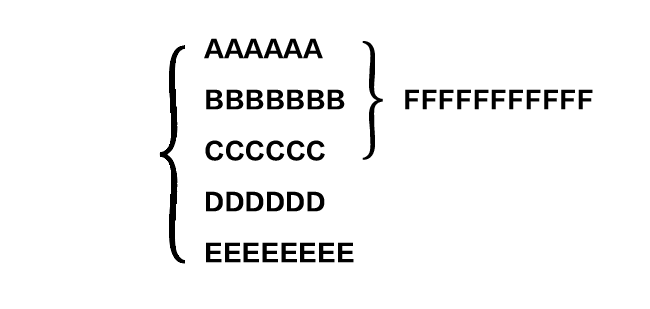
\includegraphics[width=.5\linewidth]{pic19}}
\end{qst}
\ans 可以使用aligned环境配合left, right指令.
\begin{minted}[mathescape,linenos,numbersep=5pt,gobble=0,frame=lines,framesep=2mm]{tex}
\[
  \left\{
    \begin{aligned}
      &\left.\begin{aligned}
         & AAAAAA  \\
         & BBBBBBB \\
         & CCCCCC
      \end{aligned}\right\} FFFFFFFFFF\\
      & CCCCCCCCCCCCC\\
      & DDDDDDDDDDDDD\\
      & EEEEEEEEEEEEEE
    \end{aligned}
  \right.
\]
\end{minted}
\[
  \left\{
    \begin{aligned}
       &\left.\begin{aligned}
         & AAAAAA  \\
         & BBBBBBB \\
         & CCCCCC
       \end{aligned}\right\} FFFFFFFFFF\\
       & CCCCCCCCCCCCC\\
       & DDDDDDDDDDDDD\\
       & EEEEEEEEEEEEEE
\end{aligned}
\right.
\]
也可以使用mathtools宏包的rcases环境.
\begin{mtd}
\[
  \begin{cases}
    \begin{rcases}
      AAAAAA \\ BBBBBBB \\ CCCCCC
    \end{rcases} FFFFFFFFFF\\
    CCCCCCCCCCCCC\\
    DDDDDDDDDDDDD\\
    EEEEEEEEEEEEEE
  \end{cases}
\]
\end{mtd}
\[
  \begin{cases}
    \begin{rcases}
      AAAAAA \\ BBBBBBB \\ CCCCCC
    \end{rcases} FFFFFFFFFF\\
    CCCCCCCCCCCCC\\
    DDDDDDDDDDDDD\\
    EEEEEEEEEEEEEE
  \end{cases}
\]

还可以使用multirow宏包使用表格硬凑出这样的样式.
\begin{mtd}
\[
 \begin{tabular}{r@{}c@{}l}
   & $a+b=c$ &\multirow{3}*[-0.25ex]{\scalebox{1}[1.6]{\bigg\}}}\\%
  \multirow{4}*[-0.25ex]{\scalebox{1}[2.15]{\bigg\{}} & $d+e=f$ &\\
   & $g+h=j$ &\\
   & $1+2=3$ & \\
   & $2+3=4$ &
 \end{tabular}
\]
\end{mtd}
\[
\begin{tabular}{r@{}c@{}l}
	& $a+b=c$ &\multirow{3}*[-0.25ex]{\scalebox{1}[1.6]{\bigg\}}}\\%
	\multirow{4}*[-0.25ex]{\scalebox{1}[2.15]{\bigg\{}} & $d+e=f$ &\\
	& $g+h=j$ &\\
	& $1+2=3$ & \\
	& $2+3=4$ &
\end{tabular}
\]

\begin{qst}\label{Q2018050205}
 如何生成自适应宽度的弧线和波浪线.\index{自适应弧线波浪线}
\end{qst}
\ans 可以使用stackengine宏包和scalerel宏包自定义一个指令来实现.
可以参照这样的例子:
\inputminted[fontsize=\normalsize,linenos,breaklines]{tex}{AutoFrownSim.tex}
\ifcompile\immediate\write18{xelatex AutoFrownSim.tex}\fi
\begin{center}
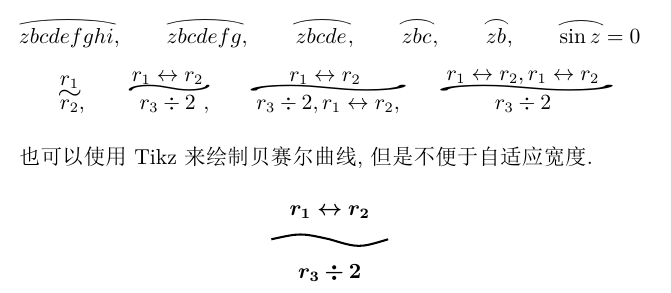
\includegraphics[width = 0.85\linewidth]{pic20}%{AutoFrownSim.pdf}
\end{center}

\end{document}